\documentclass[10pt]{beamer}
%\documentclass[10pt,handout]{beamer} % This is to create a printout!!!!!

\mode<presentation>

\usetheme{Madrid}
\definecolor{lightblue}{HTML}{5DADE2}
\usecolortheme[named=lightblue]{structure}
\setbeamercolor{button}{fg=white, bg=lightblue}
\usefonttheme[onlylarge]{structuresmallcapsserif}

\definecolor{alertcolor}{rgb}{0.8,0,0} % dark red
%\definecolor{alertcolor}{HTML}{5DADE2} % light blue
\newcommand{\hl}[1]{\textcolor{darkred}{#1}}

\renewcommand{\baselinestretch}{1.3}   
\setbeamersize{text margin left=0.5cm}
\setbeamersize{text margin right=0.5cm}

\setbeamertemplate{itemize items}[boadilla]
\setbeamertemplate{enumerate items}[default]

\usepackage[english]{babel}
\usepackage[latin1]{inputenc}
\usepackage{times}
\usepackage[T1]{fontenc}
\usepackage{graphicx}
\usepackage{appendixnumberbeamer}
\usepackage{epstopdf}

%\setbeamercovered{transparent}
\setbeamercovered{invisible}
\usenavigationsymbolstemplate{}
\usepackage{appendixnumberbeamer}

\setbeamertemplate{itemize items}[boadilla]
\setbeamertemplate{enumerate items}[default]

\title[Phillips Curve]{Phillips Curve: Structural Estimation}
\author[Nakamura-Steinsson]{Emi Nakamura \and J\'{o}n Steinsson}
\institute[Berkeley]{UC Berkeley}
\date[Oct 2021]{October 2021}

\begin{document}

\begin{frame}
  \titlepage
\end{frame}


\begin{frame}{Simple Theory}
\begin{itemize}
\itemsep1em 
\item Simple theory with Calvo pricing assumption implies:
\[ \pi_{t} = \beta E_{t} \pi_{t+1} + \lambda mc_{t} \]
where
\[ \lambda = \frac{(1-\theta)(1-\beta\theta)}{\theta} \]
and $1-\theta$ is frequency of price change, $\beta$ subjective discount factor
\item Theory implies that $mc_{t}$ is the appropriate ``forcing variable'' \\ in the Phillips curve
\item Yet most empirical work uses simple measures of the output gap \\ such as detrended output
\end{itemize}
\end{frame}

\begin{frame}{Gali-Gertler 99}
	Motivation:
	\begin{itemize}
		\itemsep1em 
		\item Is New Keynesian (Calvo) Phillips curve consistent with observed inflation persistence?
		\begin{itemize}
			\item Implies disinflations can be costless
			\item In practice, it seems disinflations are costly (Ball 94, 95) \\ (Imperfect credibility could explain this)
		\end{itemize}
		\item Do we need ``sticky inflation'' models or adaptive expectations?
		\item With quarterly data, hard to get statistically significant effect of \\ real activity on inflation, when using output gap
	\end{itemize}
\end{frame}

\begin{frame}{Simple Theory}
\begin{itemize}
\itemsep1em 
\item Under certain assumptions:
\[ mc_{t} = \kappa x_{t} \]
where $x_{t} = y_{t} - y_{t}^{n}$ denotes the output gap
\item Maybe Phillips curve estimation doesn't work because:
\begin{itemize}
\item These assumptions don't hold in reality
\item Output gap is mismeasured
\end{itemize}
\end{itemize}
\end{frame}

\begin{frame}{New Keynesian vs. Old Keynesian}
\begin{itemize}
\itemsep1em 
\item With rational expectations, NK Phillips curve can be written as
\[ \pi_{t+1} - \pi_{t} = -\lambda \kappa x_{t} + \epsilon_{t+1} \]
where $\epsilon_{t+1} = \pi_{t+1} - E_{t} \pi_{t+1}$, and assuming $\beta = 1$.
\item Traditional Phillips curve with adaptive expectations:
\[ \pi_{t} = E_{t-1} \pi_{t} + \lambda \kappa x_{t} \]
\[ \pi_{t} - \pi_{t-1} = \lambda \kappa x_{t} \]
where we are assuming $ E_{t-1} \pi_{t} = \pi_{t-1} $
\item Notice the difference in the sign on the output gap term!! \\ (and difference in timing of inflation change)
\end{itemize}
\end{frame}

\begin{frame}{New Keynesian vs. Old Keynesian}
\[ \pi_{t+1} - \pi_{t} = -\lambda \kappa x_{t} + \epsilon_{t+1} \] \vspace{-15pt}
\begin{itemize}
\itemsep1em 
\item NK Phillips curve implies tight labor market should lead inflation to fall!!
\item Theoretical logic: 
\begin{itemize}
\item Inflation is a jump variable in this model
\item When output gaps are expected, inflation should jump up and start falling
\end{itemize}
\[ \pi_{t} = \lambda \kappa \sum_{k=0}^{\infty} \beta^{k} E_{t} x_{t+k}  \]
\item I.e., inflation should lead output gap according to NK Phillips curve (Fuhrer-Moore 95)
\end{itemize}
\end{frame}

\begin{frame}{New Keynesian vs. Old Keynesian}
\begin{itemize}
\itemsep1em
\item Simple estimation using quadratically detrended log GDP yields:
\[ \pi_{t+1} - \pi_{t} = 0.081 x_{t} + \epsilon_{t+1}  \]
\item Output gap term has ``wrong sign'' (from NK perspective)
\end{itemize}
\end{frame}

\begin{frame}{Output Gap Leads Inflation}
\begin{figure}
\centering
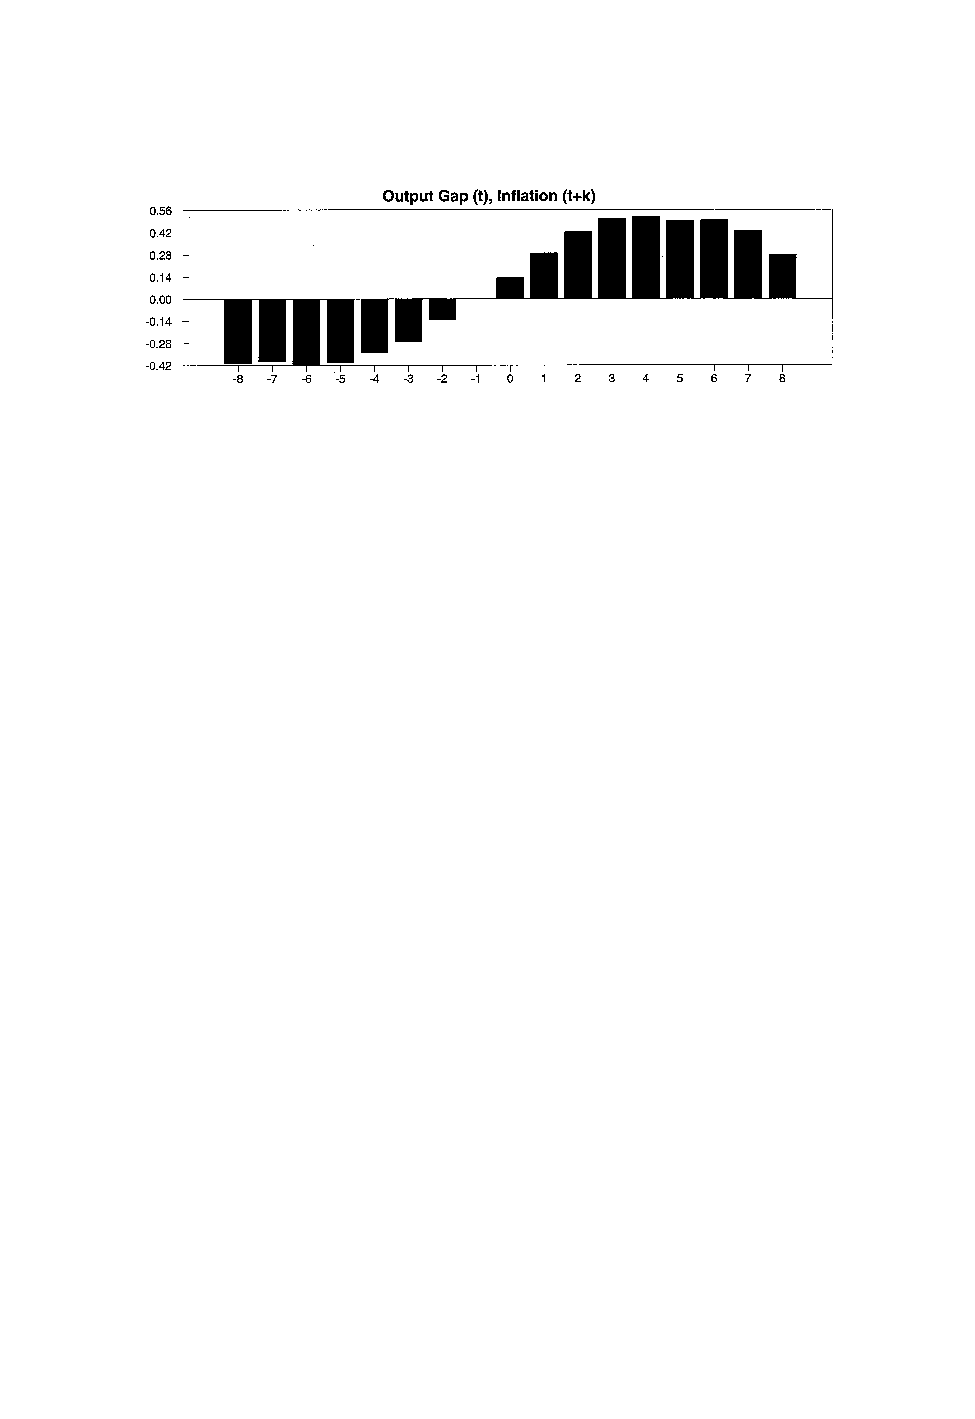
\includegraphics[height = 0.42 \textheight]{FiguresTables/GaliGertler1999Figure1A.pdf}
\end{figure}
\vspace{-0mm}
{\scriptsize Source: Gali and Gertler (1999) -- Output gap measure as detrended output using HP-filter. \\ \vspace{-5pt} Sample period 1960Q1-1997Q4. Current output gap positively correlated with \textit{future} inflation. }
\end{frame}

\begin{frame}{Marginal Cost as Opposed to Output Gap}
\begin{itemize}
\itemsep1em
\item One reaction: NK Phillips curve is empirically unrealistic.
\begin{itemize}
\item Perhaps some sluggishness messes up this jump business
\item Perhaps information frictions play a role (yield $E_{t-1} \pi_{t}$)
\end{itemize}
\item Gali-Gertler argue:
\begin{itemize}
\item Use of output gap is the problem
\item Output gap measured with error
\item Marginal costs tends to lag output gap
\end{itemize}
\item Gali-Gertler propose to estimate Phillips curve using marginal cost \\ as forcing variable
\end{itemize}
\end{frame}

\begin{frame}{Measuring Marginal Cost}
\begin{itemize}
\itemsep1em 
\item But marginal costs are unobservable as well!!
\item Gali-Gertler make following assumptions:
\begin{itemize}
\item Production function: $Y_{t} = A_{t} K_{t}^{\alpha_{k}}N_{t}^{\alpha_{n}}$
\item Labor is hired on a spot market at constant wage
\end{itemize}
\item Marginal cost:
\[ MC_{t} = \frac{W_{t}/P_{t}}{\partial Y_{t} / \partial N_{t}} = \frac{W_{t}/P_{t}}{\alpha_{n} Y_{t} / N_{t}} = \frac{1}{\alpha_{n}}\frac{W_{t}N_{t}}{P_{t}Y_{t}} = \frac{S_{t}}{\alpha_{n}} \]
proportional to labor share (average cost)
\item In logs, we get:
\[ mc_{t} = s_{t} \]
\end{itemize}
\end{frame}

\begin{frame}{Measuring Marginal Cost}
\begin{itemize}
\itemsep1em 
\item  Assumptions that Gali-Gertler make to derive this are \\ strong assumptions!!
\item Worker-firm relationship often long-term relationship
\begin{itemize}
\item Not clear that current wage is a good proxy for marginal cost
\item May just be an installment payment on a long-term contract
\item Suppose workers performs well at time $t$:
\begin{itemize}
\item  Wage may not reflect this at time $t$
\item Rather worker may expect a raise / promotion in the future
\end{itemize}
\item Firms may insure workers (labor hoarding)
\end{itemize}
\item Wages at a given point in time complicated by overtime 
\begin{itemize}
\item Marginal wage may not be the same as average wage
\end{itemize}
\end{itemize}
\end{frame}

\begin{frame}{Supply Shocks}
\begin{itemize}
\itemsep1em 
\item Gali-Gertler estimate
\[ \pi_{t} = \beta E_{t} \pi_{t+1} + \lambda s_{t} \]
\item Advantage of using measure of marginal costs:
\begin{itemize}
\item Supply shocks should be reflected in marginal costs
\end{itemize}
\end{itemize}
\end{frame}

\begin{frame}{Expectations of Inflations}
\begin{itemize}
\item What do Gali-Gertler do about expectations of inflation?
\item They assume rational expectations
\item Under this assumption, Phillips curve can be written
\[ \pi_{t} = \beta \pi_{t+1} + \lambda s_{t} + \epsilon_{t+1} \]
where $\epsilon_{t+1} = \beta E_{t} \pi_{t+1} - \beta \pi_{t+1}$ (i.i.d.)
\item They furthermore take structural model super seriously in assuming that there is \textbf{no other error term} than this expectations error
\item This strong structural assumption allows them to use lagged variables as instruments (any variable dated at time $t$ or earlier)
\end{itemize}
\end{frame}

\begin{frame}{Empirical Specification}
\begin{itemize}
\itemsep1em 
\item Maintained assumptions:
\[ \pi_{t} - \beta \pi_{t+1} - \lambda s_{t} = \epsilon_{t+1} \]
where $\epsilon_{t+1}$ is an i.i.d. expectations error and therefore uncorrelated \\ with variables at time $t$ or earlier
\item Implies:
\[ E_{t} \{ (\pi_{t} - \beta \pi_{t+1} - \lambda s_{t})z_{t} \} = 0 \]
where $z_{t}$ is in the time $t$ information set of agents
\end{itemize}
\end{frame}

\begin{frame}{Empirical Specification}

\begin{itemize}
\item Gali-Gertler use GMM with these orthogonality conditions
\[ E_{t} \{ (\pi_{t} - \beta \pi_{t+1} - \lambda s_{t})z_{t} \} = 0 \]
\item Sample period: 1960Q1-1997Q4
\item Instruments: Four lags of inflation, labor income share, output gap, long-short interest rate spread, wage inflation, and commodity price inflation (24 instruments)
\end{itemize}
\end{frame}

\begin{frame}{Why IV and not OLS?}
\[ \pi_{t} = \beta \pi_{t+1} + \lambda s_{t} + \epsilon_{t+1} \] \vspace{-15pt}
\begin{itemize}
\item Under maintained assumption that error term is i.i.d. expectation error dated at time $t+1$, instrument only needed to estimate $\beta$
\item More generally, other omitted variables (or cost push shocks) enter the equation and are dated at time $t$ (i.e., affect $\pi_{t}$):
\[ \pi_{t} = \beta \pi_{t+1} + \lambda s_{t} + \eta_{t} \]
\item In this case, both $\beta$ and $\lambda$ potentially biased
\end{itemize}
\end{frame}

\begin{frame}{Empirical Concerns}
\begin{itemize}
\itemsep1em 
\item Is $\epsilon_{t+1}$ really just an i.i.d. expectations error?
\begin{itemize}
\item If assumptions needed for $mc_{t} = s_{t}$ don't hold, it's not
\item If expectations are not rational, it is not
\end{itemize}
\item If it is not, then instruments may be invalid
\begin{itemize}
\item Slow moving omitted variables correlated with past stuff
\end{itemize}
\item 24 instruments raises concerns about many-weak instruments
\begin{itemize}
\item Many/Weak instruments issue is an overfitting issue in small samples
\item Using 24 relatively weak instruments may lead to substantial overfitting
\end{itemize}
\end{itemize}
\end{frame}

\begin{frame}{Reduced Form Results}
\begin{itemize}
\itemsep1em 
\item Estimation with labor share:
\[ \pi_{t} = \underset{(0.012)}{0.023} s_{t} + \underset{(0.045)}{0.942} E_{t} \pi_{t+1} \]
\begin{itemize}
\item Coefficients have ``correct sign'' and ``sensible'' magnitude
\end{itemize}
\item Estimation with output gap (HP-filtered GDP):
\[ \pi_{t} = - \underset{(0.005)}{0.016} s_{t} + \underset{(0.030)}{0.988} E_{t} \pi_{t+1} \]
\begin{itemize}
\item Coefficient on output gap has ``wrong sign''
\end{itemize}
\end{itemize}
\end{frame}

\begin{frame}
\begin{figure}
\centering
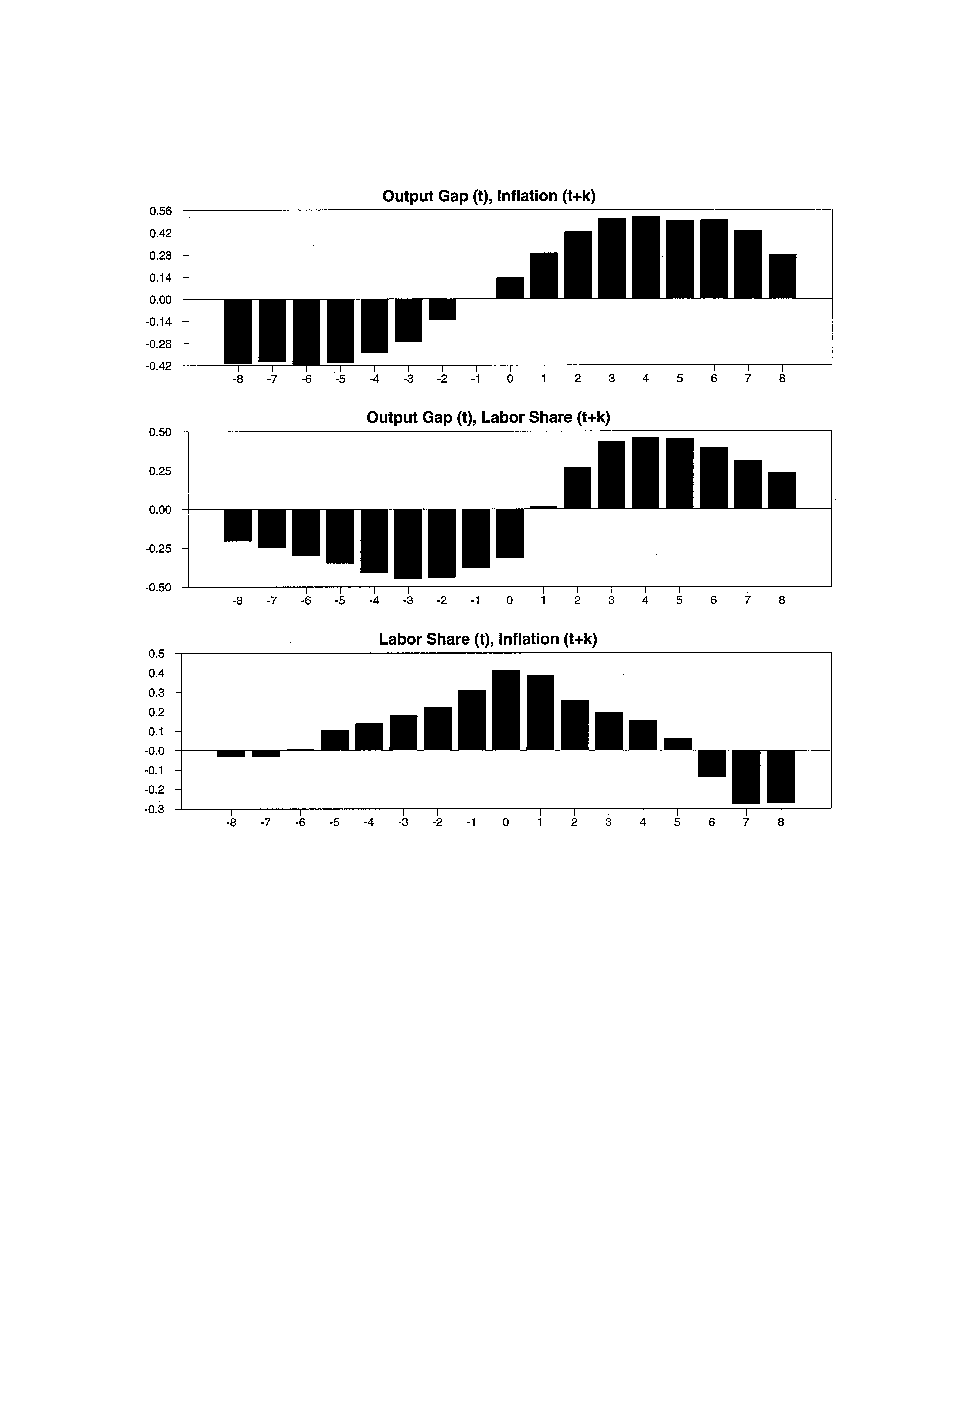
\includegraphics[height = 0.90 \textheight]{FiguresTables/GaliGertler1999Figure1.pdf}
\end{figure}
\vspace{-4mm}
{\scriptsize Source: Gali and Gertler (1999) -- Output gap measure as detrended output using HP-filter. \\ \vspace{-5pt} Sample period 1960Q1-1997Q4. }
\end{frame}

\begin{frame}{Output Gap vs. Labor Share}
\begin{itemize}
\item Output gap leads inflation in contradiction to theory
\item Labor share strongly correlated with inflation contemporaneously
\item Labor share lags output gap
\item Lag in response of labor share explains why it does better \\ in Phillips curve estimation
\end{itemize}
\end{frame}

\begin{frame}
\begin{figure}
\centering
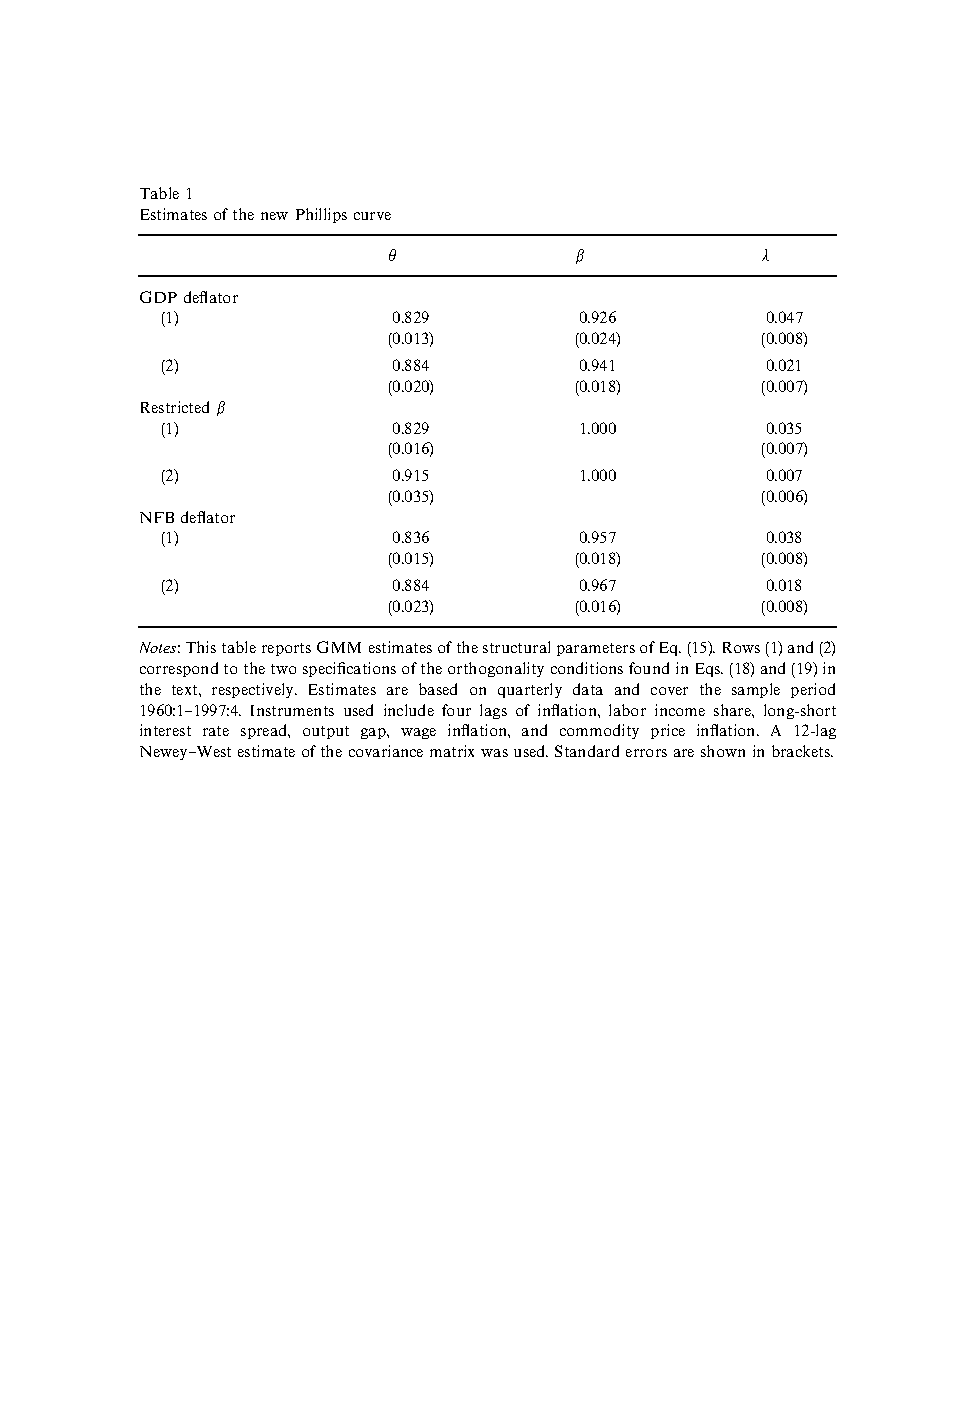
\includegraphics[height = 0.90 \textheight]{FiguresTables/GaliGertler1999Table1.pdf}
\end{figure}
\vspace{-4mm}
{\scriptsize Source: Gali and Gertler (1999) -- Two normalizations of moment conditions. }
\end{frame}

\begin{frame}{Structural Estimates}
Conparison vs. ex ante views: 
\begin{itemize}
\itemsep1em 
\item ``Sensible'' estimates for $\beta$
\item Estimates of $\theta$ on the high end
\begin{itemize}
\item Imply price rigidity of 5-6 quarters
\end{itemize}
\end{itemize}
\end{frame}

\begin{frame}{Inflation Inertia}
\begin{itemize}
\item Does NK Phillips curve account for inflation inertia?
\item Gali-Gertler estimate specification with fraction of rule-of-thumb agents
\item Rule-of-thumb agents set 
\[ p_{t}^{b} = \bar{p}_{t-1}^{*} + \pi_{t-1} \]
\item This yields

\[ \pi_{t} = \lambda mc_{t} + \gamma_{f} E_{t} \pi_{t+1} + \gamma_{b} \pi_{t-1} \]
where 
\[ \textstyle  \lambda = \frac{(1-\omega)(1-\theta)(1-\beta \theta)}{\theta + \omega[1-\theta(1-\beta)]} \]
\[ \begin{array}{lcr}  
\gamma_{f} = \frac{\beta \theta}{\theta + \omega[1-\theta(1-\beta)]} &
\hspace{0.3in} &
\gamma_{b} = \frac{\omega}{\theta + \omega[1-\theta(1-\beta)]}
\end{array} \]
and $\omega$ denotes the fraction of rule-of-thump agents
\end{itemize}
\end{frame}

\begin{frame}
\begin{figure}
\centering
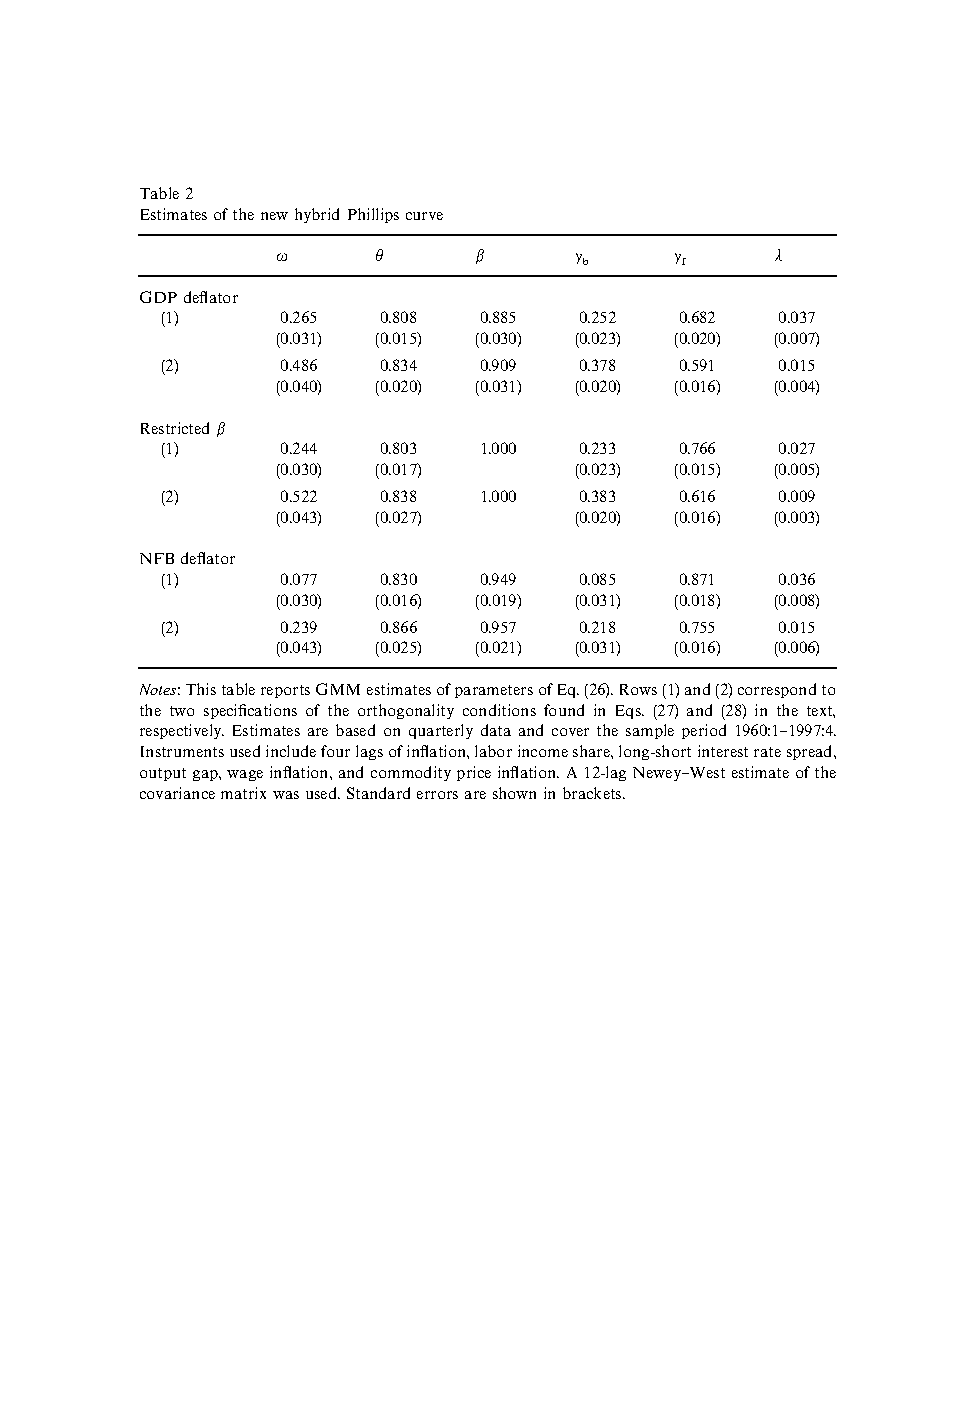
\includegraphics[height = 0.90 \textheight]{FiguresTables/GaliGertler1999Table2.pdf}
\end{figure}
\vspace{-4mm}
{\scriptsize Source: Gali and Gertler (1999) -- Two normalizations of moment conditions. }
\end{frame}

\begin{frame}{Estimation of Hybrid Phillips Curve}
\begin{itemize}
\itemsep1em 
\item Estimate of $\omega$ statistically significant
\begin{itemize}
\item Normalization 1 yields: $\omega = 0.265 (0.031)$
\item Normalization 2 yields: $\omega = 0.486 (0.040)$
\end{itemize}
\item A quarter to half of agents are rule-of-thumb
\item Gali-Gertler conclusion:
\begin{itemize}
\item Forward-looking behavior more important than backward-looking behavior
\end{itemize}
\item Estimates of $\beta$ on the low side at around 0.9
\end{itemize}
\end{frame}


\begin{frame}{Critiques of Gali-Gertler}
\begin{itemize}
\itemsep1em 
\item Subsequent work has found Gali-Gertler's results to be highly sensitive to instruments used, vintage of data, model specification
\item Mavroeidis-Plagborg-Moller-Stock 14 argue fundamental problem is weak instruments
\begin{itemize}
\item Inflation is notoriously difficult to forecast
\item Lagged variables weak instruments for future inflation
\end{itemize}
\item More recent literature has used many fewer instruments to avoid many-instruments problem
\end{itemize}
\end{frame}

\begin{frame}
\begin{figure}
\centering
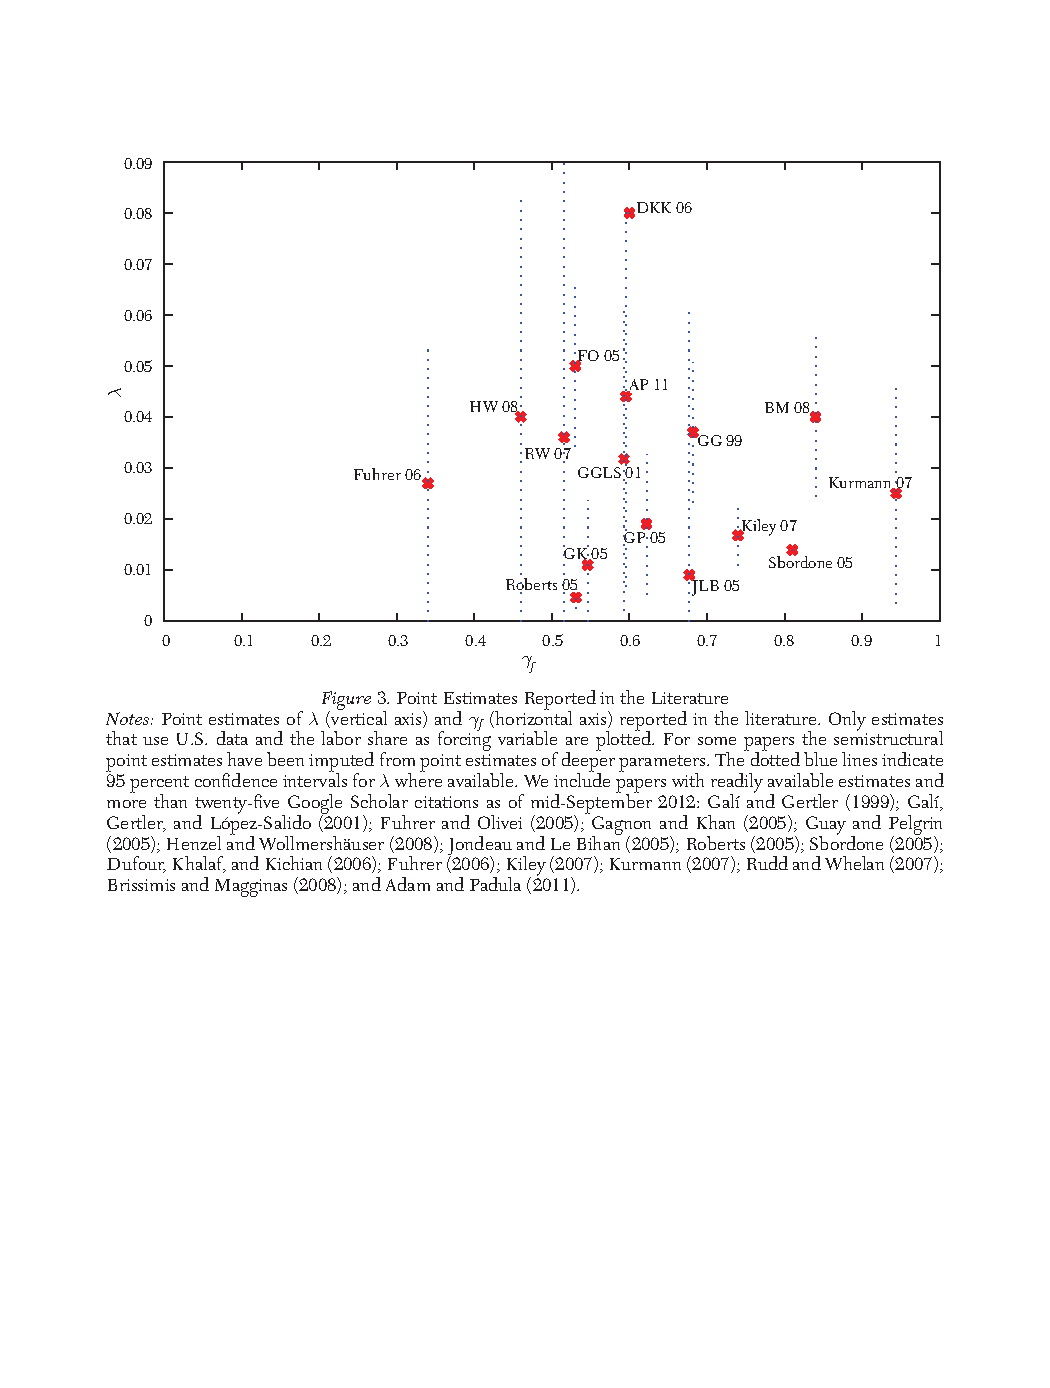
\includegraphics[height = 0.88 \textheight]{FiguresTables/MavroeidisPlagborgMollerStock2014Figure3.pdf}
\end{figure}
\vspace{-4mm}
{\scriptsize Source: Mavroeidis, Plagborg-Moller, Stock (2014) }
\end{frame}

\begin{frame}{Sensitivity to Data Vintage}
\begin{itemize}
\itemsep1em 
\item Rudd-Whelan 07 emphasize sensitivity to data vintage
\item Mavroeidis-Plagborg-Moller-Stock 14 run Gali-Gertler 99 hybrid specification with Gali-Gertler-Lopez-Salido 01 instruments on Gali-Gertler 99 sample period for two data vintages
\begin{itemize}
\item Roughly replicate Gali-Gertler 99 results for 2008 data vintage
\item With 2012 data vintage, slope of Phillips curve 30\% smaller and insignificant 
\end{itemize}
\end{itemize}
\end{frame}

\begin{frame}
\begin{figure}
\centering
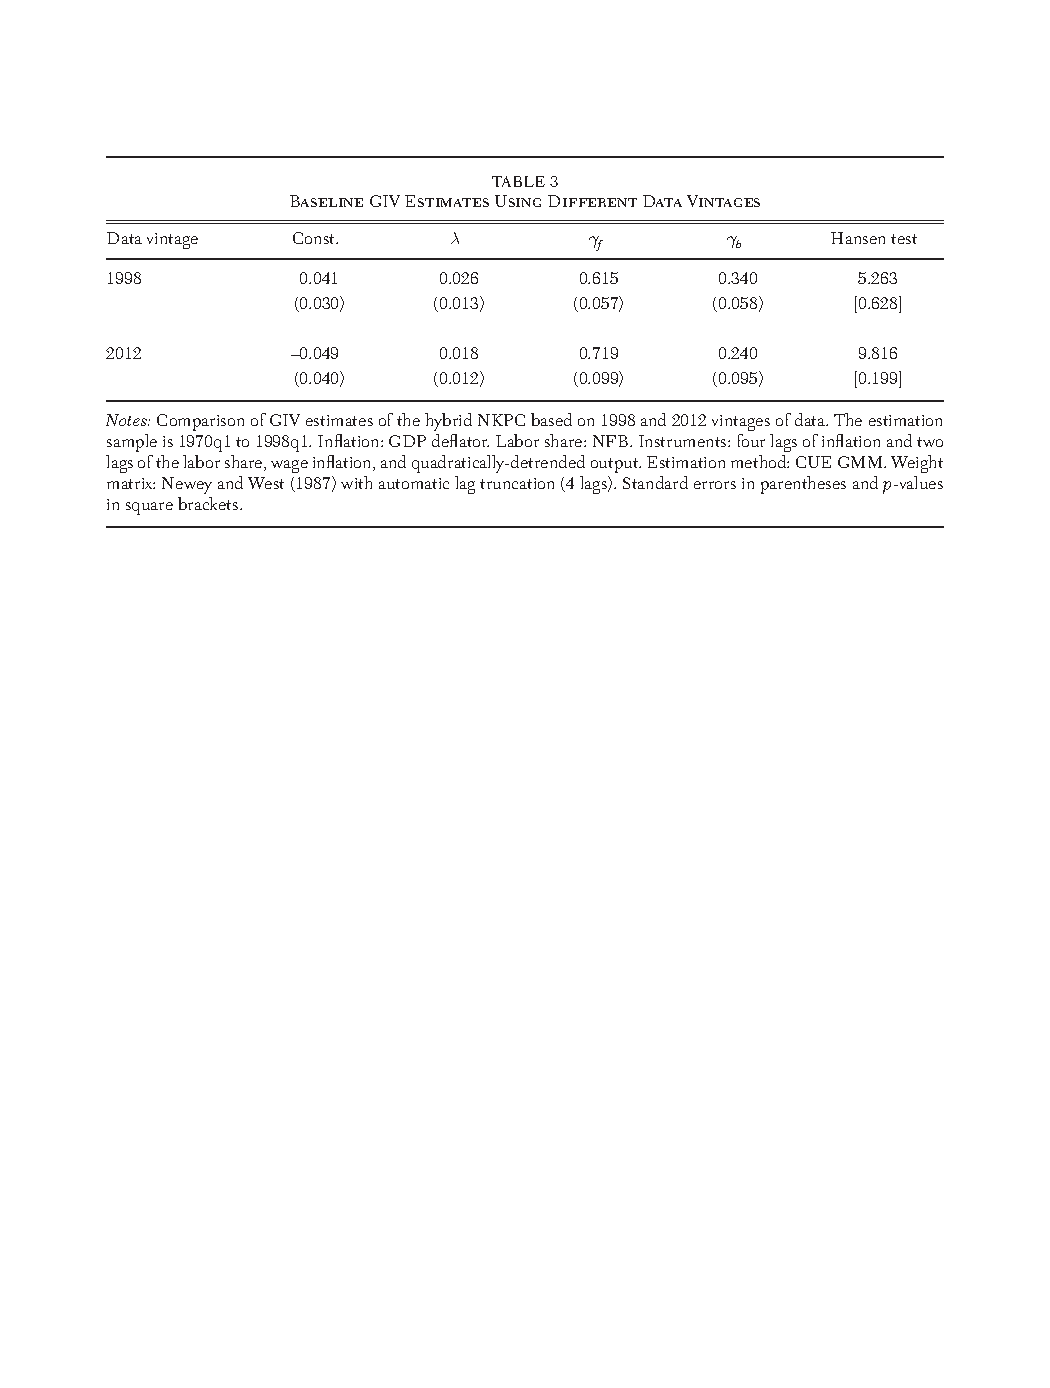
\includegraphics[height = 0.6 \textheight]{FiguresTables/MavroeidisPlagborgMollerStock2014Table3.pdf}
\end{figure}
\vspace{-0mm}
{\scriptsize Source: Mavroeidis, Plagborg-Moller, Stock (2014) }
\end{frame}

\begin{frame}{Mavroeidis, Plagborg-Moller, Stock 14}
\begin{itemize}
\itemsep1em 
\item Run huge number of different a priori reasonable specifications \\ with a common dataset 
\item Main findings:
\begin{itemize}
\item Large amount of specification uncertainty
\item Large amount of sampling uncertainty
\end{itemize}
\item Both conclusions due to weakness of identification
\end{itemize}
\end{frame}

\begin{frame}
\begin{figure}
\centering
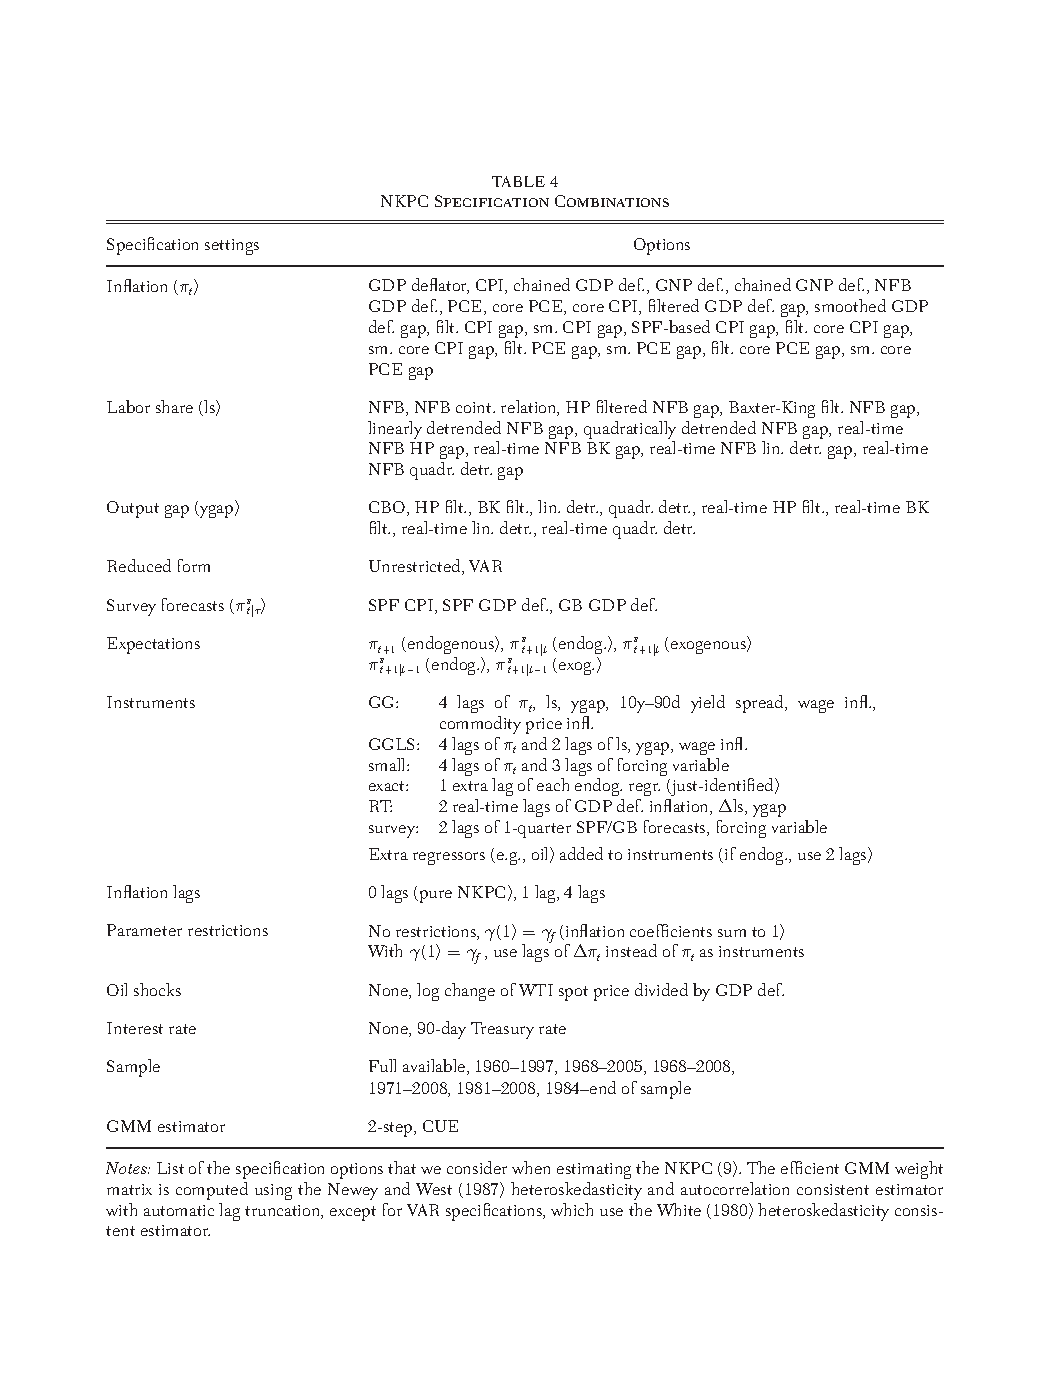
\includegraphics[height = 0.95 \textheight]{FiguresTables/MavroeidisPlagborgMollerStock2014Table4.pdf}
\end{figure}
\vspace{-5mm}
{\scriptsize Source: Mavroeidis, Plagborg-Moller, Stock (2014) }
\end{frame}


\begin{frame}{Specification Uncertainty}
\begin{figure}
\centering
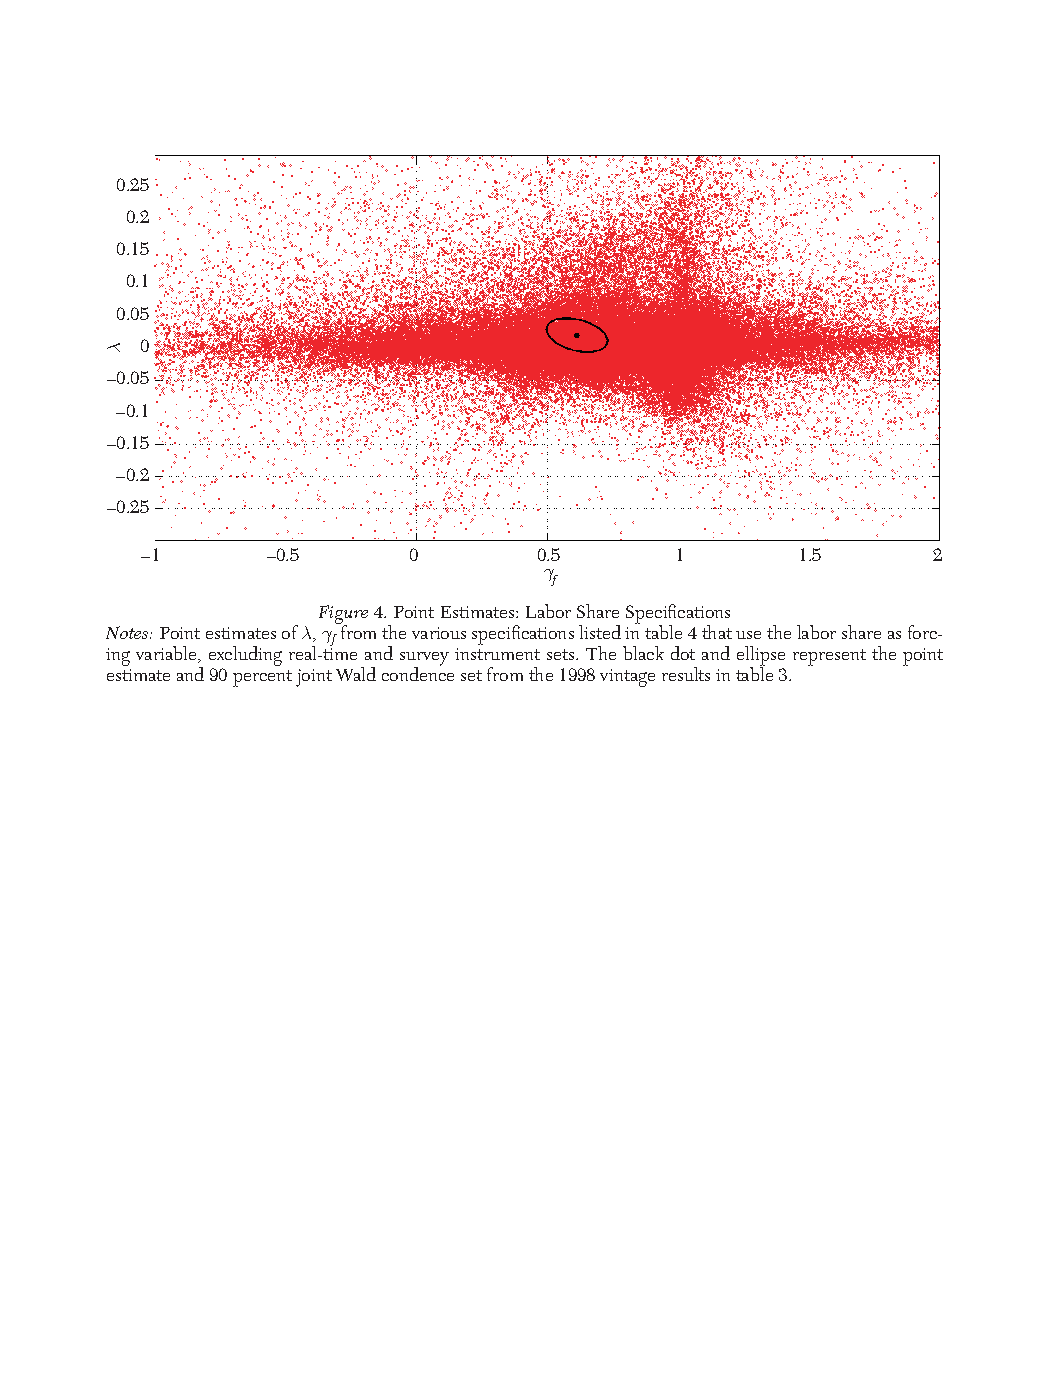
\includegraphics[height = 0.75 \textheight]{FiguresTables/MavroeidisPlagborgMollerStock2014Figure4.pdf}
\end{figure}
\vspace{-4mm}
{\scriptsize Source: Mavroeidis, Plagborg-Moller, Stock (2014) }
\end{frame}

\begin{frame}{Specification Uncertainty}
\begin{figure}
\centering
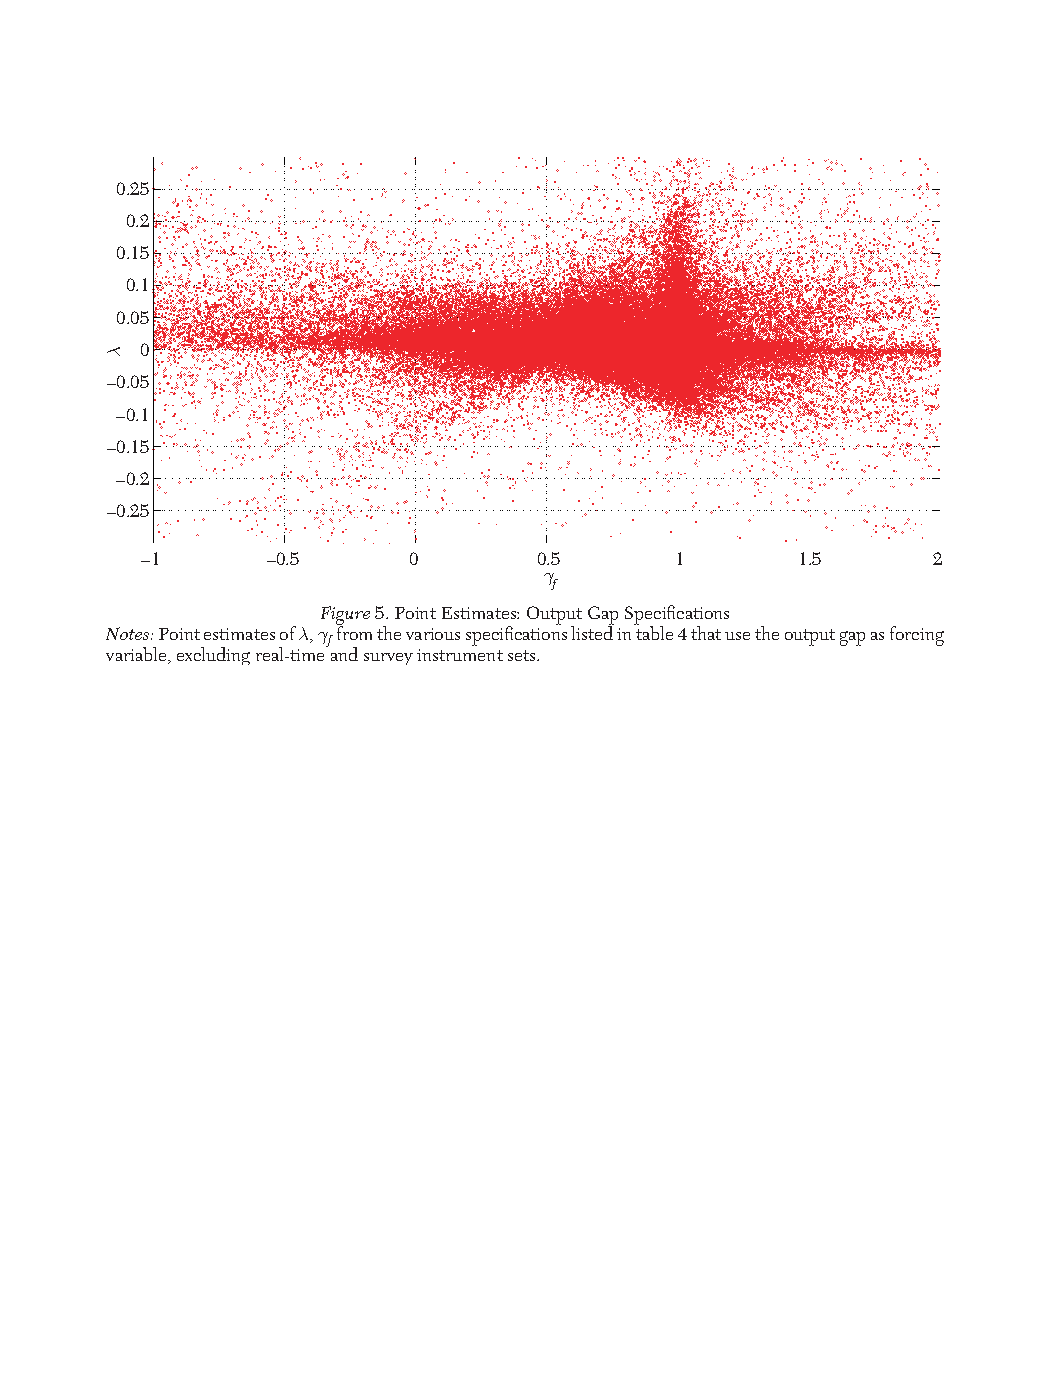
\includegraphics[height = 0.75 \textheight]{FiguresTables/MavroeidisPlagborgMollerStock2014Figure5.pdf}
\end{figure}
\vspace{-4mm}
{\scriptsize Source: Mavroeidis, Plagborg-Moller, Stock (2014) }
\end{frame}

\begin{frame}{Mavroeidis, Plagborg-Moller, Stock 14}
Overall conclusion:
\begin{itemize}
\itemsep1em 
\item[] \textit{``Literature has reached a limit on how much can be learned about the New Keynesian Phillips curve from aggregate macroeconomic time series.''}
\item[] \textit{``New identification approaches and new datasets are needed to reach an empirical consensus.''}
\end{itemize}
\end{frame}

\begin{frame}{Recent Behavior of the Labor Share}
\begin{itemize}
\itemsep1em 
\item Since about 2000, labor share has been trending downward
\item If labor share is a good measure of marginal costs, downward trend should create massive deflationary pressure \\ {\small (Coibion-Gorodichenko 15)}
\item Doesn't seem to line up with the evolution of inflation
\end{itemize}
\end{frame}

\begin{frame}
\begin{figure}
\centering
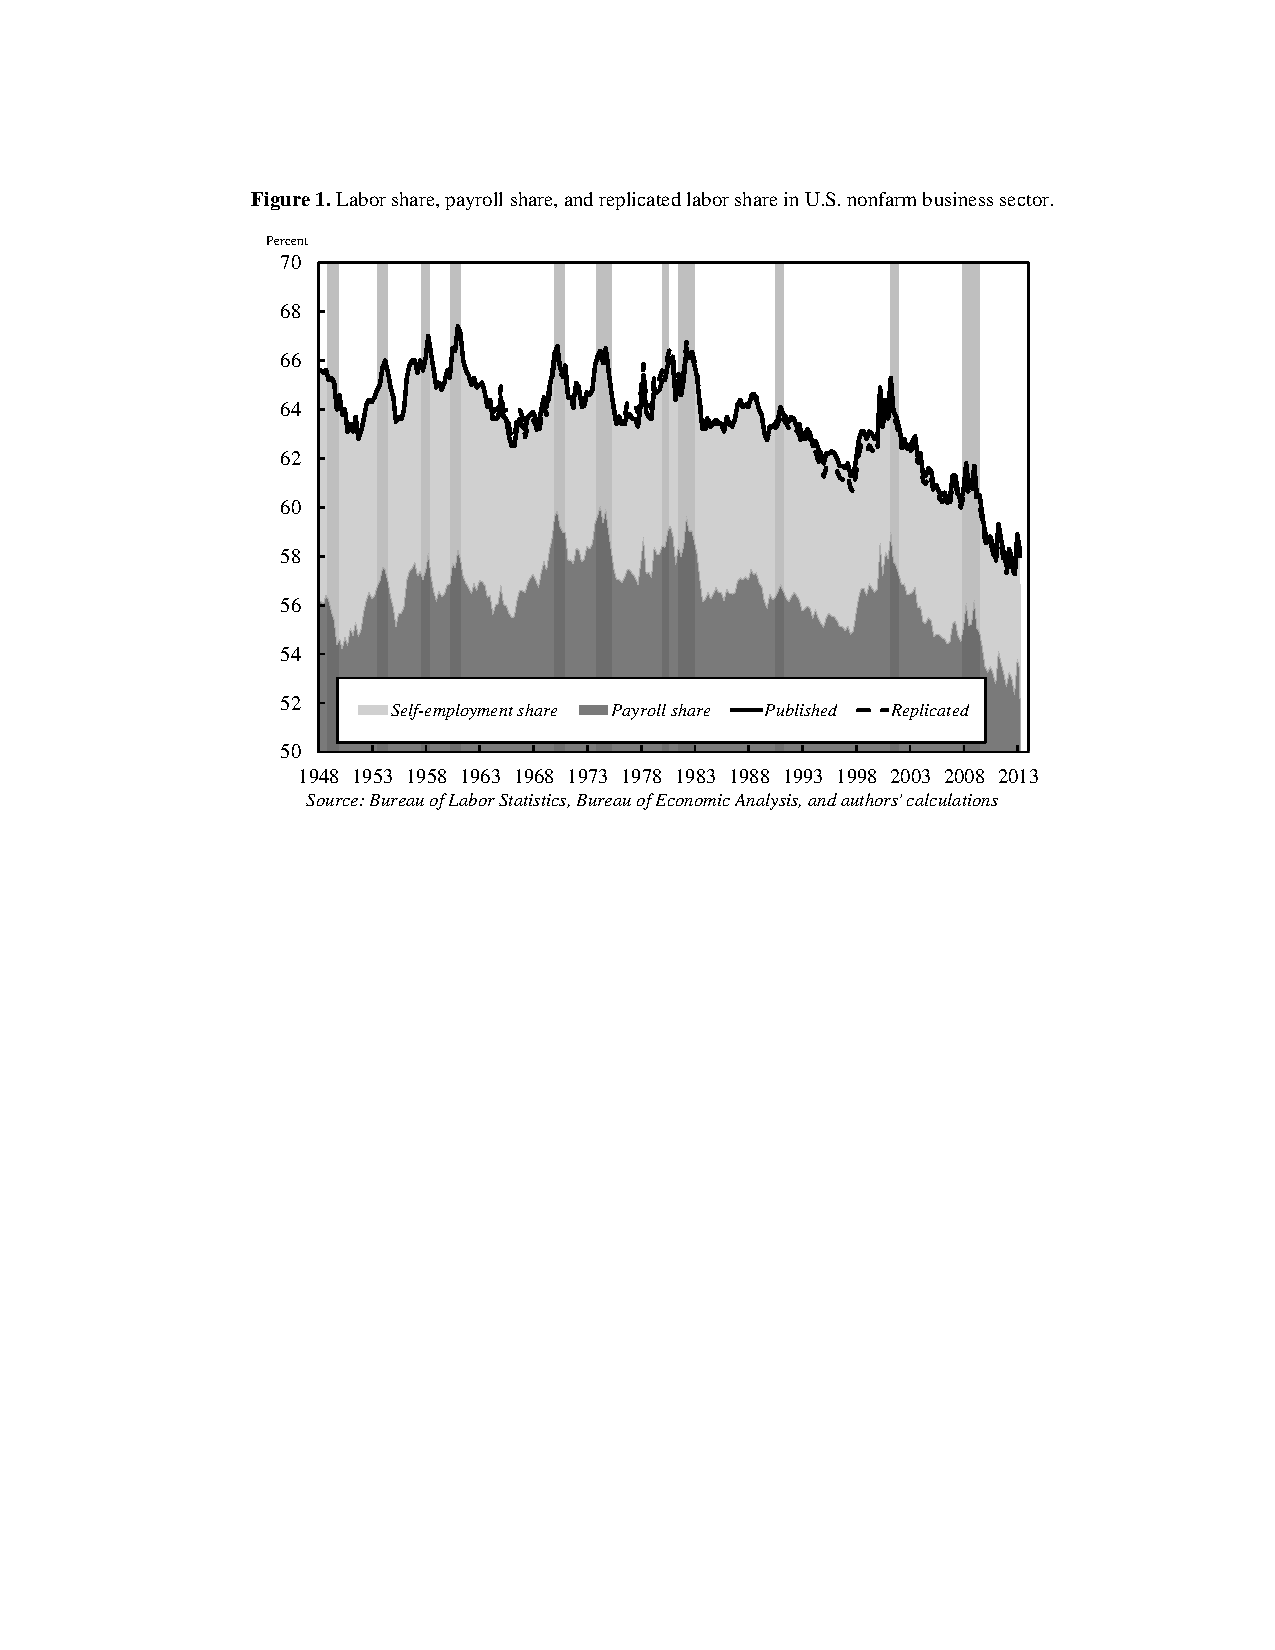
\includegraphics[height = 0.88 \textheight]{FiguresTables/ElsbyHobijnSahin2013Figure1.pdf}
\end{figure}
\vspace{-4mm}
{\scriptsize Source: Elsby, Hobijn, Sahin (2014) }
\end{frame}




\end{document}





